\section{Реализованные алгоритмы и методы визуализации}

В интеллектуальной системе реализован широкий спектр алгоритмов и методов, необходимых для обучения, визуализации и анализа моделей нейросетевой классификации, а также для работы с неполными и синтетическими данными. Приведённые ниже компоненты составляют ядро вычислительного и аналитического функционала системы.

%%%%%%%%%%%%%%%%%%%%%%%%%%%%%%%%%%%%%%%%%%%%%%%%%%%%%%%%%%%%%%%%%%%%%%%%%%%%%%%%%%%%%%%%%%%%%%%%%%%%%%%%%%%%%%%
\subsection{Многослойный персептрон}
В качестве основной вычислительной модели реализован многослойный персептрон, представленный в виде набора последовательно соединённых полносвязных слоёв. Каждый слой выполняет матрично-векторное преобразование входных признаков с последующим применением нелинейной активации. Архитектура поддерживает произвольную глубину и размерность слоёв, задаваемую пользователем.

Особое внимание уделено производительности реализации. В целях обеспечения вычислительной эффективности произведено разворачивание вложенных циклов~\cite{huang1999generalized} и оптимизация операций умножения с использованием предварительного выделения буферов. Все операции реализованы в терминах низкоуровневых операций над типизированными массивами~\cite{matsakis2014typed} JavaScript, без применения сторонних библиотек.

%%%%%%%%%%%%%%%%%%%%%%%%%%%%%%%%%%%%%%%%%%%%%%%%%%%%%%%%%%%%%%%%%%%%%%%%%%%%%%%%%%%%%%%%%%%%%%%%%%%%%%%%%%%%%%%
\subsection{Оптимизационные алгоритмы}
Для обучения нейросетевых моделей реализованы различные варианты стохастического градиентного спуска:

\begin{itemize}
    \item SGD -- базовый метод без накопления импульса;
    \item SGD с импульсом (momentum) -- учитывает направление предыдущих градиентов;
    \item Adam -- использует адаптивную нормализацию градиентов на основе скользящих средних;
    \item Adamax, Adagrad, RMSprop, Adadelta~\cite{zeiler2012adadelta} — альтернативные адаптивные модификации~\cite{ruder2016overview}, отличающиеся способами обновления весов.
\end{itemize}

Каждый из алгоритмов может быть выбран пользователем, параметры (скорость обучения, размер пакета) доступны для настройки в пользовательском интерфейсе.

%%%%%%%%%%%%%%%%%%%%%%%%%%%%%%%%%%%%%%%%%%%%%%%%%%%%%%%%%%%%%%%%%%%%%%%%%%%%%%%%%%%%%%%%%%%%%%%%%%%%%%%%%%%%%%%
\subsection{Функции потерь}
Система поддерживает несколько типов функций потерь, применяемых как для задач классификации, так и регрессии:

\begin{itemize}
    \item Среднеквадратичная ошибка (MSE);
    \item Средняя абсолютная ошибка (MAE);
    \item Потеря Хубера~\cite{meyer2021alternative} (Huber loss);
    \item Логарифмическая гиперболическая косинус-функция~\cite{saleh2022statistical} (Log-Cosh).
\end{itemize}

Функции потерь реализованы вручную, с учётом числовой устойчивости и эффективности вычислений.

%%%%%%%%%%%%%%%%%%%%%%%%%%%%%%%%%%%%%%%%%%%%%%%%%%%%%%%%%%%%%%%%%%%%%%%%%%%%%%%%%%%%%%%%%%%%%%%%%%%%%%%%%%%%%%%
\subsection{Объясняющее двоичное дерево}
Для анализа принятия решений реализован алгоритм построения объясняющего двоичного дерева. Дерево формируется по реальным выходам модели на имеющихся данных, без рассмотрения всех гипотетических состояний пространства (что позволяет избежать экспоненциального роста сложности). Структура дерева отображается в виде таблицы ячеек, с указанием статистических характеристик.

%%%%%%%%%%%%%%%%%%%%%%%%%%%%%%%%%%%%%%%%%%%%%%%%%%%%%%%%%%%%%%%%%%%%%%%%%%%%%%%%%%%%%%%%%%%%%%%%%%%%%%%%%%%%%%%
\subsection{Визуализация модели и метрик}
Визуализация является ключевой частью интеллектуальной системы машинного обучения. Реализованы следующие возможности:

\begin{itemize}
    \item Построение выходной поверхности модели (в двумерном или трёхмерном виде) с применением различных цветовых схем (рисунок~\cref{fig:vis_model_output}), а также иерархическое разбиение пространства на ячейки (рисунок~\cref{fig:vis_cells}).
    \item Отображение архитектуры модели, включая весовые коэффициенты и их градиенты на каждом слое.
    \item Графики метрик (ошибки регрессии, классификации, доли отказов) на обучающих и тестовых выборках (рисунок~\cref{fig:vis_metrics_hist}\subcaptionref{fig:vis_metrics_hist_metrics}).
    \item Гистограммы распределения выходных значений модели по каждому из классов и фону (рисунок~\cref{fig:vis_metrics_hist}\subcaptionref{fig:vis_metrics_hist_hist}).
\end{itemize}

\begin{figure}[ht]
    \centerfloat{
        \hfill
        \subcaptionbox{Линейный режим}{
            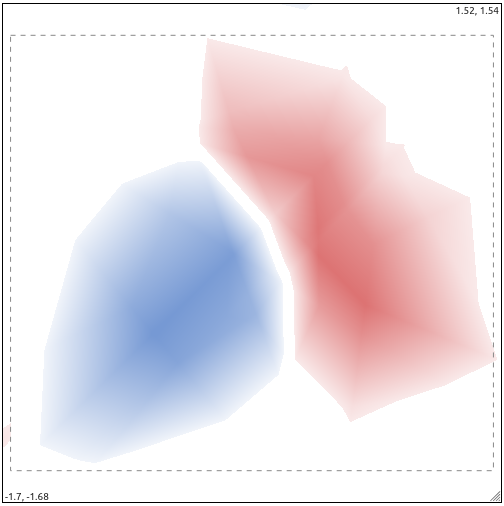
\includegraphics[width=0.24\linewidth]{Dissertation/images/ch4/algorithms_and_visualizations/model_output_linear.png}}
        \hfill
        \subcaptionbox{Дискретный режим}{
            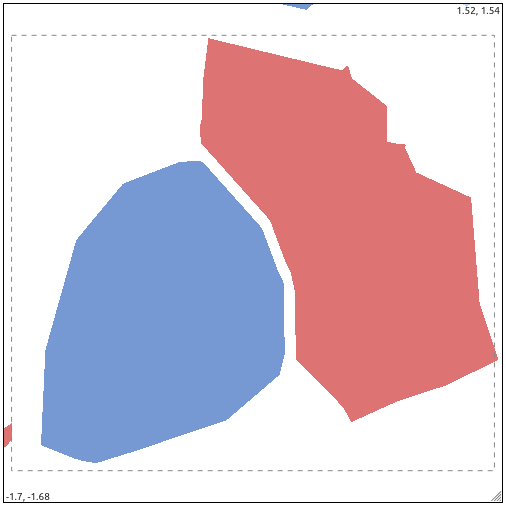
\includegraphics[width=0.24\linewidth]{Dissertation/images/ch4/algorithms_and_visualizations/model_output_discrete.png}}
        \hfill
        \subcaptionbox{Дискретный режим на 10 уровней}{
            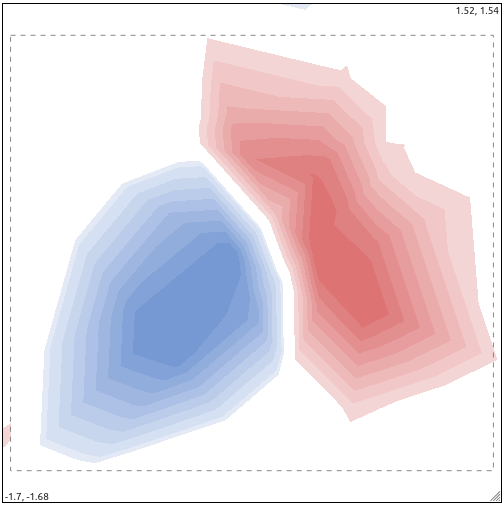
\includegraphics[width=0.24\linewidth]{Dissertation/images/ch4/algorithms_and_visualizations/model_output_discrete10.png}}
        \hfill
        \subcaptionbox{3D режим}{
            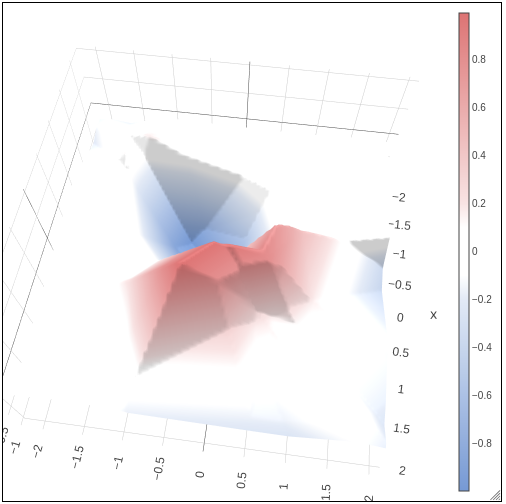
\includegraphics[width=0.24\linewidth]{Dissertation/images/ch4/algorithms_and_visualizations/model_output_3d.png}}
        \hfill
    }
    \caption{Визуализация выхода модели}
    \label{fig:vis_model_output}
\end{figure}

\begin{figure}[ht]
    \centerfloat{
        \hfill
        \subcaptionbox{Ячейки первого скрытого слоя}{%
            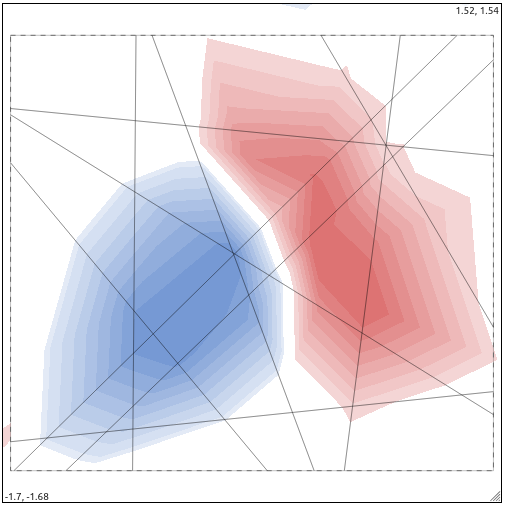
\includegraphics[width=0.3\linewidth]{Dissertation/images/ch4/algorithms_and_visualizations/cells1.png}}
        \hfill
        \subcaptionbox{Ячейки второго скрытого слоя}{%
            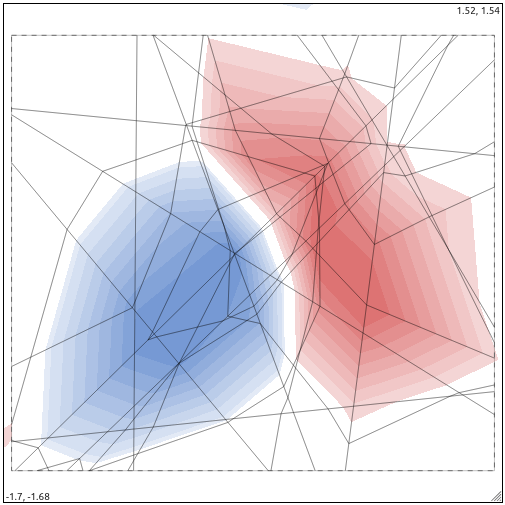
\includegraphics[width=0.3\linewidth]{Dissertation/images/ch4/algorithms_and_visualizations/cells2.png}}
        \hfill
        \subcaptionbox{Ячейки выходного слоя}{%
            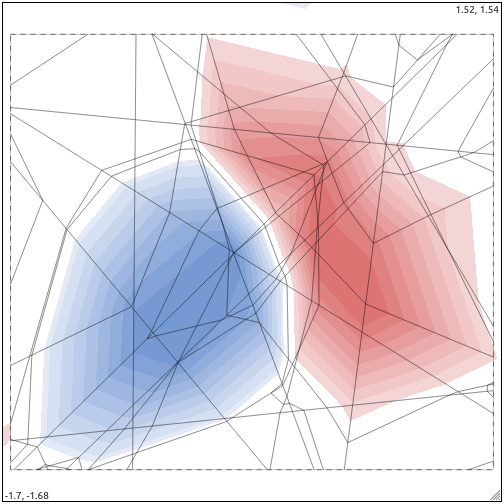
\includegraphics[width=0.3\linewidth]{Dissertation/images/ch4/algorithms_and_visualizations/cells3.png}}
        \hfill
    }
    \caption{Визуализация иерархического разбиения на ячейки}
    \label{fig:vis_cells}
\end{figure}

\begin{figure}[ht]
    \centerfloat{
        \hfill
        \subcaptionbox{Метрики\label{fig:vis_metrics_hist_metrics}}{%
            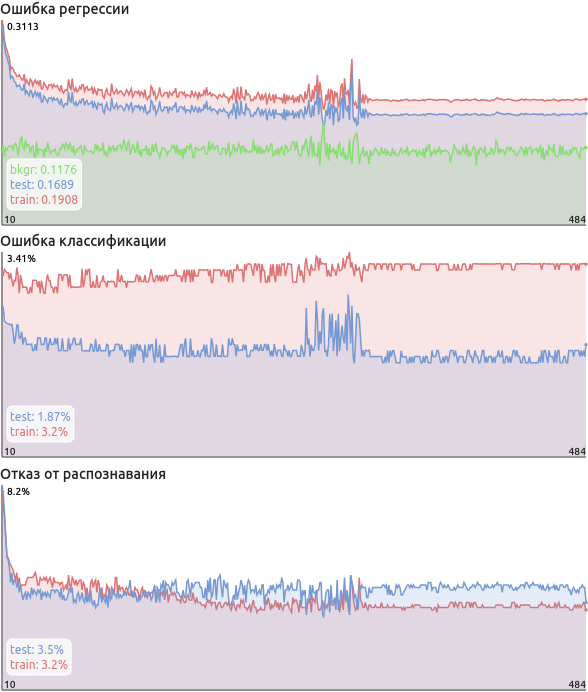
\includegraphics[width=0.4\linewidth]{Dissertation/images/ch4/algorithms_and_visualizations/metrics.png}}
        \hfill
        \subcaptionbox{Гистограммы выхода модели\label{fig:vis_metrics_hist_hist}}{%
            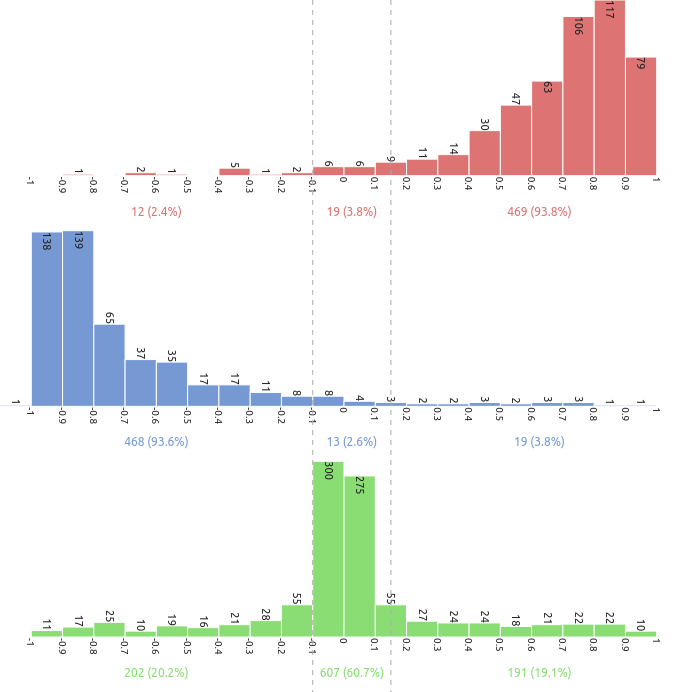
\includegraphics[width=0.59\linewidth]{Dissertation/images/ch4/algorithms_and_visualizations/histograms.png}}
        \hfill
    }
    \caption{Визуализация метрик и гистограмм распределения выхода персептрона на обучающих данных}
    \label{fig:vis_metrics_hist}
\end{figure}

Для генерации графических представлений используются встроенные средства Canvas API и SVG с ручной реализацией всех визуальных компонентов. Визуализация обновляется в реальном времени по мере обучения модели. Для трёхмерного отображения выхода модели используется единственная внешняя зависимость Plotly.js~\cite{sievert2021package}.

%%%%%%%%%%%%%%%%%%%%%%%%%%%%%%%%%%%%%%%%%%%%%%%%%%%%%%%%%%%%%%%%%%%%%%%%%%%%%%%%%%%%%%%%%%%%%%%%%%%%%%%%%%%%%%%
\subsection{Анализ отказов от классификации}
Оценка надёжности классификации осуществляется с использованием порогового механизма, основанного на параметре доверия \(\beta\). При выходном значении, не превышающем порог \(\beta\), модель отказывается от классификации, помечая объект как нераспознанный. Это позволяет существенно повысить доверие к решениям, принятым моделью, особенно в задачах с высокой ценой ошибки.

Реализована визуализация распределения отказов: гистограммы выходных значений и графики зависимости доли отказов и точности от выбранного порога.

%%%%%%%%%%%%%%%%%%%%%%%%%%%%%%%%%%%%%%%%%%%%%%%%%%%%%%%%%%%%%%%%%%%%%%%%%%%%%%%%%%%%%%%%%%%%%%%%%%%%%%%%%%%%%%%
\subsection{Генерация и модификация данных}
Система включает инструменты генерации заранее подготовленных наборов данных для обучения и тестирования (рисунок~\cref{fig:vis_data}). Пользователь может настраивать следующие параметры:

\begin{itemize}
    \item Размер обучающей и тестовой выборки и их соотношение.
    \item Пропорции (баланс) классов.
    \item Доля ошибочно размеченных наблюдений.
    \item Нормализация, стандартизация и масштабирование признаков.
\end{itemize}

\begin{figure}[ht]
    \centerfloat{
        \hfill
        \subcaptionbox{набор данных ``Спираль``}{%
            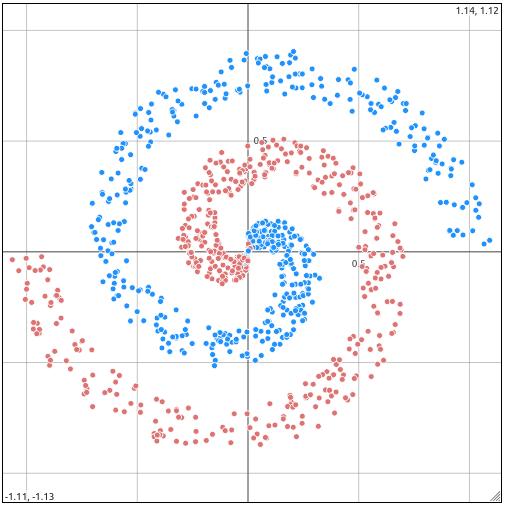
\includegraphics[width=0.24\linewidth]{Dissertation/images/ch4/algorithms_and_visualizations/data_spiral.png}}
        \hfill
        \subcaptionbox{набор данных ``Окружность``}{%
            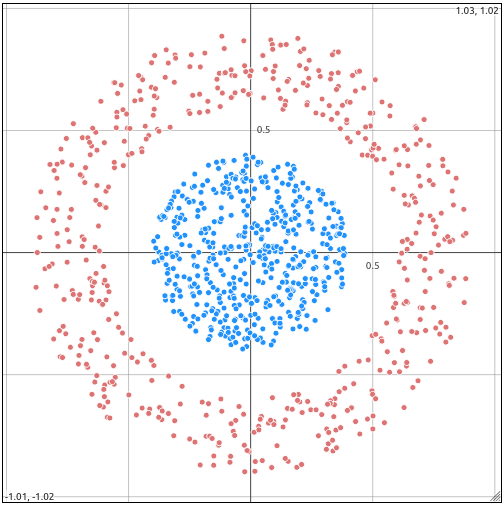
\includegraphics[width=0.24\linewidth]{Dissertation/images/ch4/algorithms_and_visualizations/data_circle.png}}
        \hfill
        \subcaptionbox{набор данных ``Moons``}{%
            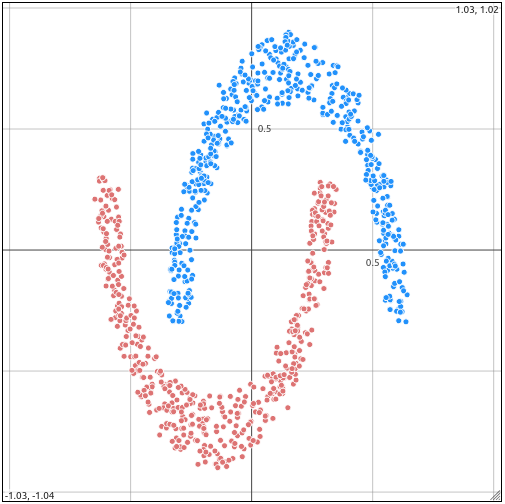
\includegraphics[width=0.24\linewidth]{Dissertation/images/ch4/algorithms_and_visualizations/data_moons.png}}
        \hfill
        \subcaptionbox{набор данных ``Гауссианы``}{%
            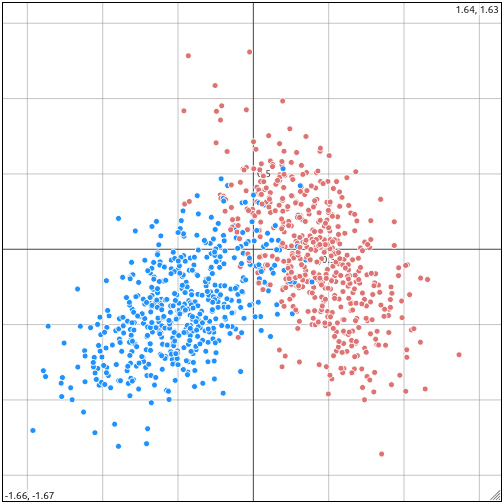
\includegraphics[width=0.24\linewidth]{Dissertation/images/ch4/algorithms_and_visualizations/data_gaussians.png}}
        \hfill
    }
    \caption{Примеры наборов данных, доступных в интеллектуальной системе}
    \label{fig:vis_data}
\end{figure}
